We have now introduced the main principles of Bayesian inference. Now, we can
turn to the Kalman filter, a popular and widely used algorithm for state 
estimation. The Kalman filter (KF, for short) is a recursive algorithm that uses
Bayesian inference to estimate the state of a dynamic system based on a sequence
of noisy measurements.

The key feature of the KF is the ability to predict future states of the system.
This is essential for applications that require to foresee the behavior of
tracked objects before the state of these objects is measured. Examples of such
systems may include autonomous driving or air defence systems. The prediction 
ability helps also to overcome situations when a sensor fails to measure the
position of an object (a so-called misdetection).

In the following subsections, we will introduce the state-space models, give
a formal definition of a general Bayes filter, infer the Kalman filter formulas
and discuss the Constant Velocity (CV) model, a common motion model used in the
Kalman filter.

\subsection{Multivariate Gaussian Distribution}
    Before we start learning the basics of Bayesian filtration, we should extend our knowledge of the Gaussian distribution to the multidimensional case. As mentioned in Section \ref{sec:gauss}, it plays a very important role in object tracking and, in particular, in this work. Formulas and theorems defined in this section are essential for defining and proving the Kalman filter formulas. We will define several properties of multivariate Gaussians required later.

First, we define the multivariate Gaussian distribution with mean vector $\boldsymbol\mu$, covariance matrix $\Sigma$, and evaluated at $\mathbf{x}$ as:

\begin{equation}\label{eq:vec-gauss-def}
    \mathscr{N}\left(\mathbf{x} ; \mathbf\mu, \mathbf\Sigma\right)
    = \frac{1}{\sqrt{(2\pi)^n|\mathbf{\Sigma}|}}\exp\left(-\frac{1}{2}(\mathbf{x}-\boldsymbol{\mu})^\top \mathbf{\Sigma}^{-1} (\mathbf{x}-\boldsymbol{\mu})\right),
\end{equation}

where $n$ is the length of the vector $\mathbf{x}$, and $|\cdot|$ denotes the determinant of a matrix. 

The multivariate Gaussian distribution is a generalization of the univariate Gaussian distribution, where instead of a single mean and variance, we have a mean vector and a covariance matrix that characterizes the correlation between the variables. Note that the exponent contains the expression known as the Mahalanobis distance, which we will encounter throughout this work. It is given by:

\begin{definition}[Mahalanobis distance]\label{def:mahalanobis}
    For vectors $\mathbf x$ and $\mathbf y$ and the symmetrical positive-definite matrix $\mathbf S$, the Mahalanobis distance is defined as:

    \begin{equation}
        d(\mathbf x, \mathbf y) 
        = \sqrt{
            (\mathbf x - \mathbf y)^\intercal
            \mathbf{S}^{-1}
            (\mathbf x - \mathbf y)
        }.
    \end{equation}
\end{definition}

As we will later see, in object tracking, we heavily use conditional probabilities, and in particular, conditioning and marginalization of joint distributions of Gaussian random variables. Thus, we define the following two theorems.

\begin{theorem}[Conditioning on a Gaussian joint distribution]\label{theorem:gauss-cond}
    Let $\mathbf{x}$ and $\mathbf{y}$ be Gaussian random variables with distributions $\mathscr{N}\left(\mathbf{x} ; \mathbf\mu_x, \mathbf\Sigma_{xx}\right)$ and $\mathscr{N}\left(\mathbf{y} ; \mathbf\mu_y, \mathbf\Sigma_{yy}\right)$, respectively. Let their joint probability be given by:

    \begin{equation*}
        p(\mathbf{x}, \mathbf{y}) = \mathscr{N}\left(
            \begin{bmatrix}
                \mathbf{x} \\
                \mathbf{y}
            \end{bmatrix};
            \begin{bmatrix}
                \boldsymbol\mu_x \\
                \boldsymbol\mu_y
            \end{bmatrix},
            \begin{bmatrix}
                \mathbf{\Sigma}_{xx} & \mathbf{\Sigma}_{xy} \\
                \mathbf{\Sigma}_{xy}^\intercal & \mathbf{\Sigma}_{yy}
            \end{bmatrix}
        \right).
    \end{equation*}
    Then the conditional distribution of $\mathbf{x}$ given $\mathbf{y}$ is defined as:
    \begin{equation}\label{eq:gauss-cond}
        p(\mathbf{x}|\mathbf{y}) =
        \mathscr{N}\left(\mathbf{x}; \boldsymbol\mu_{x|y}, \mathbf\Sigma_{x|y}\right),
    \end{equation}
    where
    \begin{align}
        \boldsymbol\mu_{x|y}
        &= \boldsymbol\mu_x + \mathbf{\Sigma}_{xy} \mathbf{\Sigma}_{yy}^{-1}(\mathbf{y} - \boldsymbol\mu_y) \\
        \mathbf\Sigma_{x|y} 
        &= \mathbf\Sigma_{xx} - \mathbf\Sigma_{xy}\mathbf\Sigma_{yy}^{-1}\mathbf\Sigma_{xy}^\intercal.\label{eq:gauss-cond-params}
    \end{align}
\end{theorem}

\begin{theorem}[Marginalization of a Gaussian joint distribution]\label{theorem:gauss-marg}
    Consider the same $\mathbf{x}$, $\mathbf{y}$, $\mathscr{N}\left(\mathbf{x} ; \mathbf\mu_x, \mathbf\Sigma_{xx}\right)$, $\mathscr{N}\left(\mathbf{y} ; \mathbf\mu_y, \mathbf\Sigma_{xx}\right)$ and $p(\mathbf{x}, \mathbf{y})$ given in Theorem \ref{theorem:gauss-cond}. The marginal distribution of $x$ is defined as:

    \begin{equation*}
        p(\mathbf{x}) = \mathscr{N}\left(\mathbf{x} ; \mathbf\mu_x, \mathbf\Sigma_{xx}\right).
    \end{equation*}
\end{theorem}

The proofs for Theorem \ref{theorem:gauss-cond} and Theorem \ref{theorem:gauss-marg} can be found in classical statistical textbooks such as \cite[161--163]{johnsonAppliedMultivariateStatistical2007}.

\subsubsection{Gaussian mixtures}

In multi-target tracking, the posterior density cannot be described in a simple Gaussian distribution. Generally, the posterior distribution can have any form with only assumption that the integral of it sums to one. However, when we are dealing with Gaussian-linear cases, the posterior density is often represented as a mixture of many Gaussian components. A Gaussian mixture is a linear combination of multiple Gaussian distributions and its pdf is expressed in the following way:

\begin{equation}\label{eq:gaussian-mixture}
    p(\mathbf{x}) = \sum_{i=1}^N w_i \mathscr{N}\left(\mathbf{x}; \boldsymbol{\mu}_i, \Sigma_i\right),
\end{equation}

where $N$ is the number of Gaussian components in the mixture, $w_i$ is the weight of the $i$th component, the weights $w_i \geq 0$ sum to one, i.e. $\sum_{i=1}^N w_i = 1$, and each component $\mathscr{N}\left(\mathbf{x}; \boldsymbol{\mu}_i, \Sigma_i\right)$ is a Gaussian distribution with the mean in $\boldsymbol{\mu}_i$ and the covariance matrix $\Sigma_i$. An example of a Gaussian mixture pdf is illustrated in Figure \ref{fig:gaussian-mixture}.

\begin{figure}
\centering
  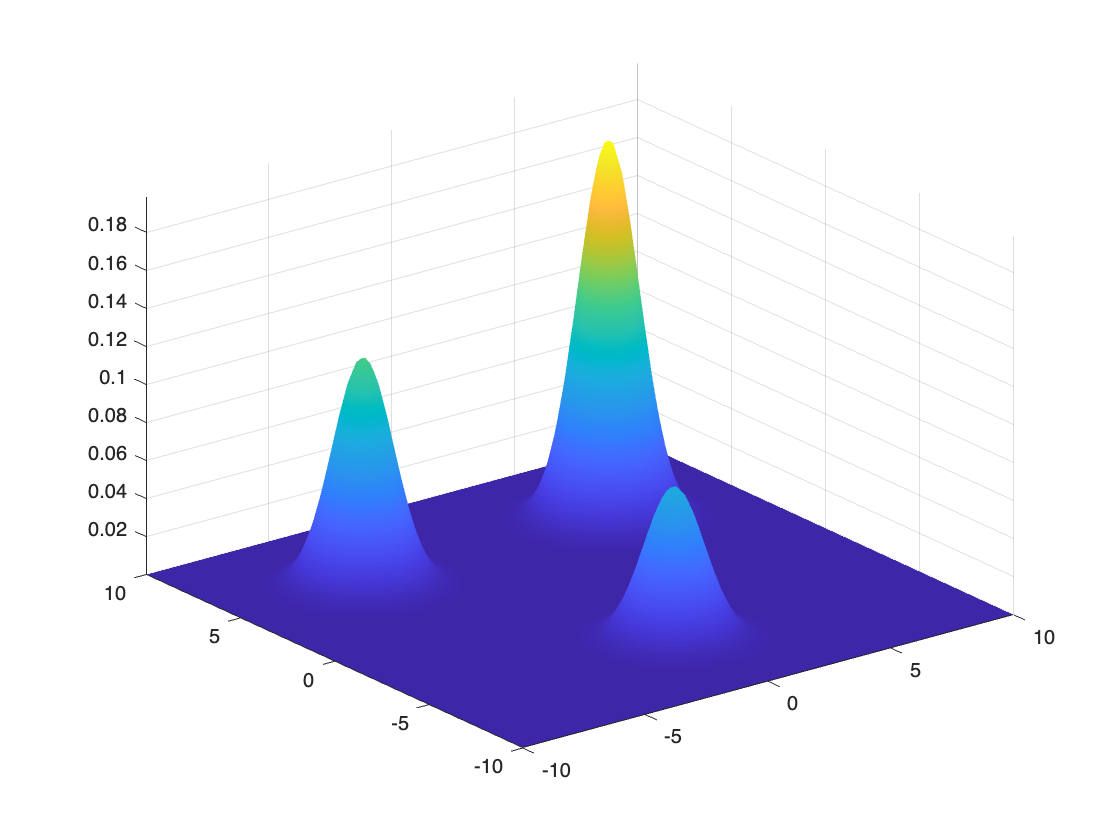
\includegraphics[width=.4\linewidth]{figures/gaussian-mixture.png}
  \caption{An example of a Gaussian mixture with three components. The first component is centered at $[0, -5]^\intercal$ with weight $0.2$, the second component has mean in $[-5, 5]^\intercal$ with weight $0.3$ and the last has mean $[5, 5]^\intercal$ and the weight $0.5$.}
  \label{fig:gaussian-mixture}
\end{figure}

Since the weights sum to one, the Gaussian mixture satisfies the normalization requirement of pdfs and is thus a valid probability density function itself. The weights in the mixture represent the relative importance of the corresponding component. Gaussian mixtures are used to model complex distributions and have several nice mathematical properties as the Gaussian distribution, as we will later see. That is why Gaussian mixtures are widely used to represent posterior distributions in many MTT filters. Moreover, one can easily approximate any distribution with a Gaussian mixture using algorithms such as the Expectation-Maximization algorithm.

A mixture $f(\mathbf{X})$ with $N$ components will have the expected value $\boldsymbol{\hat{\mu}}$ and the covariance $\hat{\Sigma}$ according to the following equations:

\begin{align}
    \boldsymbol{\hat{\mu}} &= \sum_{i=1}^N w_i \boldsymbol{\mu}_i, \\
    \hat{\Sigma} &= \sum_{i=1}^N w_i \Sigma_i + \Tilde{\Sigma},
\end{align}

where the term $\Tilde{\Sigma}$ is called the spread-of-the-innovations and is defined as:

\begin{equation}
    \Tilde{\Sigma}= \sum_{i=1}^N
        w_i (\boldsymbol{\mu}_i - \hat{\boldsymbol{\mu}})
        (\boldsymbol{\mu}_i - \hat{\boldsymbol{\mu}})^\intercal.
\end{equation}

The spread-of-the-innovations quantifies the magnitude of the difference between expectations of individual components.

\subsection{State-space model}\label{sec:state-model}
    
In the previous section, we established the relationships between prior and 
posterior distributions and learned about recursive Bayesian estimation of the 
posterior. Now, we will explore these concepts in the context of object 
tracking.

Object tracking involves estimating the internal states of objects that move in 
some space, which are often unknown to us. These states may include physical 
properties of objects such as position, velocity, acceleration, and 
orientation, depending on the application. Sensors such as cameras, infrared 
scanners, lidars or radars constantly generate measurements of the object 
states, which may be the distance of an object to the sensor, or its 
temperature. However, these measurements are often noisy due to environmental 
conditions or imperfections of the sensor. We use Bayesian filtering to 
estimate the real state of the objects and filter out the noise.

To handle the complexity and diversity of possible situations and properties, 
we need a systematic framework for modeling object motion that captures all 
sources of uncertainty and the nature of physical behavior of objects. This 
framework is called state-space modeling. In state-space models, the internal 
state we want to estimate is represented as a vector of variables that evolve 
over time according to a set of rules specified by the \textit{motion model}, 
which is a known function. The measurements obtained at each time step are 
modeled as a different function of the state variables, known as the 
\textit{measurement model}\footnote{
    It should be mentioned that the names `motion' and `measurement' models are 
    not the only terms used to describe them. The reader may also encounter 
    terms such as kinematic, state-transition, dynamic, or system models for the 
    motion model, and terms like observation, sensor, or likelihood models for 
    the measurement model. All of these names are correct, and their use depends 
    on the context in which they are applied. However, in this work, the author 
    strives for consistency and will use the terms `motion' and `measurement' 
    models throughout the entire text.
}.

For example, consider a moving bicycle and a surveillance camera with a 
rectangular field of view (FoV). The bicycle enters the FoV and crosses it at a 
constant speed. The camera has an algorithm that estimates the position of 
objects in the space from the image. With each frame $f$, it returns a new 
position, say $(\hat x_f, \hat y_f)$. We can represent the state of the bicycle 
as a vector of the position and velocity, which are unknown variables. Based on 
the measurements, we estimate their values using the known physical relation 
between distance, velocity, and time: $d = v \Delta t$, where $d$ is the 
distance that the object with velocity $v$ traveled in time $\Delta t$.

Both the motion and measurement models should include some noise. In the 
example above, the movement of the bicycle cannot perfectly follow the formula, 
and there will always be some minor changes in speed. Moreover, the measurement 
model, which translates an estimated state into a measurement, will also 
contain some uncertainty since the camera does not have a perfect 
representation of the space.

We can now describe these models formally. Note that since the state is a 
vector, we will use $\mathbf{x}$ for vectors. The motion and measurement models 
can be generally expressed as:

\begin{align*}
    p(\vecat{x}{k} | \vecat{x}{k-1}) 
        &= f_t(\vecat{x}{k-1}, \vecat{u}{k}, \vecat{w}{k}), \\
    p(\vecat{z}{k} | \vecat{x}{k}) 
        &= h_t(\vecat{x}{k}, \vecat{v}{k}),
\end{align*}

where $f_t$ and $h_t$ are functions, $\vecat{x}{k-1}$ is the estimated state 
from time step $k-1$, $\vecat{u}{k}$ is called the input (or control) vector, 
and $\vecat{w}{k}$ and $\vecat{v}{k}$ are zero-mean noise random variables.

However, this definition is too general since the functions $f_t$ and $h_t$ can 
be anything. As mentioned earlier, to get a closed-form solution in the 
Bayesian inference framework, we need to choose conjugate distributions for the 
likelihood and the prior. The Kalman filter, which we will describe soon, works 
for the Gaussian-linear case, where the functions $f_t$ and $h_t$ are linear 
and noise variables are distributed as Gaussian, i.e., 
$\vecat{w}{k}, \vecat{v}{k} \sim \mathscr{N}(\mathbf{0}, \Sigma)$. The Gaussian-
linear state-space model has the following representation:

\begin{align}
    p(\vecat{x}{k} | \vecat{x}{k-1}) 
        &= \mathbf{F} \vecat{x}{k-1}
            + \mathbf{B} \vecat{u}{k}
            + \vecat{w}{k},
        & \vecat{v}{k} \sim \mathscr{N}(\mathbf{0}, \mathbf{Q}), \\
    p(\vecat{z}{k} | \vecat{x}{k})
        &= \mathbf{H} \vecat{x}{k} + \vecat{v}{k},
        & \vecat{w}{k} \sim \mathscr{N}(\mathbf{0}, \mathbf{R}), \\
    p(\vecat{x}{0}) &\sim \mathscr{N}(\vecat{\hat{x}}{0}), \vecat{P}{0}),&
\end{align}

where:

\begin{itemize}
    \item $\mathbf{F}$ is the \textit{transition matrix},
    \item $\mathbf{B}$ is the \textit{input matrix},
    \item $\mathbf{H}$ is the \textit{measurement matrix},
    \item $\mathbf{Q}$ and $\mathbf{R}$ are symmetric positive definite matrices
        that describe the statistical properties of the motion noise
        \vecat{v}{k} and the measurement noise \vecat{w}{k}, respectively,
    \item $\vecat{\hat x}{0}$ and $\vecat{P}{0}$ are mean and variance of the 
    prior state.
\end{itemize}

The control variable $\vecat{u}{k}$, in general, represents some input signal from the environment, and $\mathbf{B}$ specifies how the input signal affects the dynamic system. This may include the effect of gravity on the vertical traveled distance or the voltage applied to some circuit. However, in object tracking, we rely on measurements obtained from sensors to update our estimate of the object's state. We do not have control over the object's motion. Thus, the input matrix is often redundant, and we omit it (or set it to a zero matrix) along with the input variable $\vecat{u}{k}$.

The notation above may be inconvenient in some cases. In this work, we will often use a shorter version that has the same meaning:

\begin{align}
    p(\vecat{x}{k} | \vecat{x}{k-1})
        &= \mathscr{N}(\vecat{x}{k}; \mathbf{F}\vecat{x}{k-1}, \mathbf{Q}), 
        \label{eq:motion-model} \\
    p(\vecat{z}{k} | \vecat{x}{k})
        &= \mathscr{N}(\vecat{z}{k}; \mathbf{H}\vecat{x}{k}, \mathbf{R}), 
        \label{eq:measurement-model} \\
    \vecat{x}{0}
        &\sim \mathscr{N}(\vecat{x}{0}; \vecat{\hat{x}}{0}, \vecat{P}{0}).
        \label{eq:prior-x0}
\end{align}

\subsubsection{Constant Velocity Model}\label{sec:cv-model}

The Constant Velocity (CV) model is one of the most commonly used motion and measurement models in the context of object tracking. It describes the kinematics of objects in a 2D space that move with a constant velocity. The state vector comprises a position vector and a velocity vector, and while the position vector contains the coordinates of the object in the space, the velocity vector contains the object's speed in the direction of each axis.

The CV model is linear and one of the simplest models. It assumes that the speed of objects remains unchanged during tracking, with only small deviations from the constant. This model can be reasonably utilized in scenarios where objects do not change their speed or direction, such as vehicles on highways or planes in the sky. Since the state vector contains only four variables, the use of this model does not increase the computational burden on tracking algorithms.

The motion equation for the CV model is given by \ref{eq:motion-model}, and the state vector $\vecat{x}{k}$, the state transition matrix $\mathbf{F}$, and the process noise matrix $\mathbf{Q}$ can be defined as:

\begin{equation}
    \vecat{x}{k} =
    \begin{bmatrix}
        x_{1,k} \\ 
        x_{2,k} \\ 
        v_{x_1,k} \\ 
        v_{x_2,k}
    \end{bmatrix};
    \quad
    \mathbf{F} =
    \begin{bmatrix}
       1 & 0 & dt & 0 \\
       0 & 1 & 0 & dt \\
       0 & 0 & 1 &  0 \\
       0 & 0 & 0 &  1 
    \end{bmatrix};
    \quad
    \mathbf{Q} = q^2 \cdot
    \begin{bmatrix}
        \frac{dt^3}{3}    & 0                 & \frac{dt^{2}}{2}  & 0  \\
        0                 & \frac{dt^3}{3}    & 0                 & \frac{dt^{2}}{2} \\
        \frac{dt^{2}}{2}  & 0                 & dt                & 0 \\
        0                 & \frac{dt^{2}}{2}  & 0                 & dt
    \end{bmatrix},
\end{equation}

where $dt$ is the change in time between the last estimation and the newly computed one, and $q$ is the motion noise parameter, which represents the uncertainty in the state transition.

The measurement model transforms a state vector from the state space into the measurement space. Since the vanilla Kalman filter, which we will derive soon, works only with linear models, the measurement model for the CV model assumes sensors measurements in the same 2D space as in the state vectors. The measurement equation is given by \ref{eq:measurement-model}, and the measurement matrix $\mathbf{H}$ and the measurement noise matrix $\mathbf{R}$ can be defined as:

\begin{equation}
    H =
    \begin{bmatrix}
        1 & 0 &0 & 0 \\
        0 & 1 &0 & 0
    \end{bmatrix};
    \quad
    R =
    r^{2}\cdot
    \begin{bmatrix}
        1 & 0 \\
        0 & 1
    \end{bmatrix},
\end{equation}

where $r$ is the measurement noise parameter, which determines the variance of the measurement noise.

We need to describe the choice of parameters $q$ and $r$ in more detail. These parameters are crucial in obtaining good estimates from a filter. These parameters are not known a priori and their values should be chosen carefully by the means of trial and error, or using automated methods like, for instance, in \cite{bulutProcessMeasurementNoise2011}. However, selecting appropriate values often involves a trade-off between tracking accuracy and computational complexity, and the use of exact methods depends on the application and one's requirements.

The CV model can be extended with additional information, such as change of speed. In this way we will come to the constant acceleration model. However, it will not be used in this work and, therefore, we will not leave formal definition of this model here.


\subsection{The Bayes filter}\label{sec:bayes-filter}

We have learned how the internal state of a system can be represented in terms
of a state vector and motion and measurement models. Now, we are ready to 
present the formal definition of the Bayes filter, the general abstraction of
any Bayesian filter, including the Kalman filter and the PHD filter.

First, we need to make a very important assumption on states. This assumption
is called the \textit{Markov model property}. This property states that, for 
the motion model, the present state of a system $x_k$ is dependent only on 
the state on the previous time step $x_{k-1}$ given all past states $x_{1:k-1}$ 
and measurements $z_{1:k-1}$. More formally:

\begin{equation}
p(x_k | x_1, \ldots, x_{k-2}, x_{k-1},
        z_1, \ldots, z_{k-2}, z_{k-1}) 
    = p(x_k | x_{k-1}).
\end{equation}

A similar requirement must hold for measurement model, that is:

\begin{equation}
    p(z_k | x_1, \ldots, x_{k-2}, x_{k-1}, x_{k}
        z_1, \ldots, z_{k-2}, z_{k-1}) 
    = p(z_k | x_k).
\end{equation}

The Markov property may seem restrictive but in reality it is not because state-
space models allows us to capture dependencies in the system dynamics by simply 
introducing more variables into the state vector. For instance, if we have a 
system where the current state has a dependence on the previous two states, we 
can augment the state vector to include the last two states as variables, and 
the Markov property will still hold.

The Bayes filter uses the motion and measurement models and assumes that this
property holds. The Bayes filter is a recursive framework that estimates an
internal state of the system over time using measurements. Every iteration of
the filter consists of two steps: prediction and update. On the prediction step,
the filter estimates a internal state $x_k$ based on the previous state
$x_{k-1}$ and the motion model $p(x_k | x_{k-1})$. The prediction step
is also known as the Chapman-Kolmogorov equation.

\begin{theorem}[The prediction step. The Chapman-Kolmogorov equation]\label{theorem:bayes-filter-predict}\label{theorem:chapman-kolmogorov}
    Given the set of measurements $z_{1:k-1} = \{z_1, z_2, \ldots, z_{k-1}\}$ 
    and the current state $x_{k-1}$ and the motion model $p(x_k | x_{k-1})$, 
    the prediction step of the Bayes filter is computed as follows:

    \begin{equation}
        p\left({x}_k | {z}_{1: k-1}\right)
        = \int 
            p\left(
                {x}_k, {x}_{k-1} | {z}_{1: k-1}
            \right)
            \mathrm{d} {x}_{k-1}
        = \int
            p\left(
                {x}_k | {x}_{k-1}\right
            ) p\left(
                {x}_{k-1} | {z}_{1: k-1}
            \right)
            \mathrm{d} {x}_{k-1}.
    \end{equation}
\end{theorem}

Next, on the update step, the filter corrects the predicted state with the 
measurement $z_k$ using the measurement model $p(z_k | x_k)$. This step is
computed using the standard Bayes' rule.

\begin{theorem}[The update step]\label{theorem:bayes-filter-update}
    Given the output of the prediction step of the Bayes filter 
    $p\left({x}_k | {z}_{1: k-1}\right)$, the observed measurement $z_k$
    and the measurement model $p(z_k | x_k)$, the update step of the Bayes
    filter is computed as follows:
    
    \begin{equation}
        p\left({x}_k | {z}_{1: k}\right)=\frac{p\left({z}_k | {x}_k\right) p\left({x}_k | {z}_{1: k-1}\right)}{p\left({z}_k | {z}_{1: k-1}\right)} \propto p\left({z}_k | {x}_k\right) p\left({x}_k | {z}_{1: k-1}\right).
    \end{equation}
\end{theorem}

These two steps create a loop, and to use the filter, we first predict the next state using the Chapman-Kolmogorov equation, and then we update our guess with a measurement. Note, that we will often use the simplified notation to explicitly state the time step of the value. The notation $\vecat{\cdot}{k|k-1}$ represents the predicted value at time step $k$, and the notation $\vecat{\cdot}{k|k}$ represents the updated value at time step $k$ after incorporating a measurement.

Now, having introduced the general Bayes filter, we will continue with 
exploring the Kalman filter in detail, the popular and widely used tool for 
state estimation.

\subsection{The Kalman filter}

The Kalman filter is one of the most well-known and widely used algorithms in 
signal processing and control theory. It is a recursive algorithm that allows 
the estimation of internal states of entities in dynamic systems from a set of 
measurements that may be noisy or missing at some time steps. The filter was 
proposed by Rudolf Kalman in 1960 \cite{kalmanNewApproachLinear1960} and has 
since been pervasively used to control a vast array of consumer, health, 
commercial, and defense products \cite{grewalApplicationsKalmanFiltering2010}.

The development of the filter was motivated by the need to improve aerospace 
technology in the United States during the Cold War between the Soviet Block 
and the North American Treaty Organization. Because the Soviet Union managed to 
launch its artificial satellites and successfully send a human to space, the 
federal government of the United States supported research into new 
technologies in the aerospace area.

The Kalman filter is an example of a general Bayes filter that was introduced 
earlier. This means that the filter estimates the posterior distribution of the 
internal state at discrete time steps using prior information about the 
observed object's state and a set of noisy measurements. As briefly mentioned 
in Section \ref{sec:state-model}, the Kalman filter works on state-space linear 
models with Gaussian noise and a Gaussian prior of the state. The predict-
update loop in the Kalman filter is the same as in the Bayes filter, and the 
same Chapman-Kolmogorov equation defined in \ref{theorem:chapman-kolmogorov} 
and the update equation defined in \ref{theorem:bayes-filter-update} are 
incorporated.

The main advantage of the Kalman filter is that it allows for the estimation of 
the state of a system in real-time. It handles noisy measurements well and is 
fast; however, it is sensitive to initial parameter settings, such as the noise 
covariance matrices \cite{gePerformanceAnalysisKalman2016}. Nonetheless, there 
are new methods being developed that propose mechanisms to overcome this 
drawback, as in \cite{matiskoNoiseCovariancesEstimation2010} and 
\cite{yuenOnlineEstimationNoise2013}.

One of the main drawbacks of the Kalman filter is its Gaussian-linear 
assumption. In real-world applications, many systems exhibit non-linearity, and 
the Kalman filter may be ineffective. Nonetheless, several extensions of the 
filter have been proposed that address this. Two well-known algorithms are the 
Unscented Kalman Filter (UKF) and the Extended Kalman filter (EKF). The UKF is 
an algorithm that uses a set of carefully chosen sigma points to capture the 
true mean and covariance of the predicted and updated distributions without 
the need for linearization \cite{wanUnscentedKalmanFilter2000}. The EKF, on 
the other hand, linearizes the nonlinear motion and measurement models using a 
first-order Taylor expansion \cite{smithApplicationStatisticalFilter1962}. 
These methods have been proven to be effective in many applications, including 
the PHD filter. However, they are beyond the scope of this thesis and will not 
be covered in detail.

\subsubsection{The Gaussian identity}

Before we introduce the actual formulas of the Kalman filter, we should introduce a new fundamental theorem in object tracking and then deduce a corollary from it. These will also be used later when we infer formulas for the the GM-PHD filter. We define this theorem using a general notation without any meaning for Bayesian filters to avoid the confusion of variables when we use this theorem in different parts of different filters.
\todo{when finished, make the notation bold}

\begin{theorem}[The Gaussian product identity]\label{theorem:gaussian-identity}
    Given matrices and vectors $A, U, m, d$, and $V$ of appropriate dimensions, and that $U$ and $V$ are positive definite, the following identity applies:

    \begin{equation}\label{eq:gid}
        \mathscr{N}(x ; A y + d, U) \mathscr{N}(y ; m, V)=\mathscr{N}(x ; A m + d, U + A V A^\intercal) \mathscr{N}(y ; \hat{m}, \hat{V}),
    \end{equation}

    where
    \begin{align}
        \hat{m} & = m + K (y - Am - d), \\ 
        \hat{V} & = (I - K A) V, \\
        K &= V A^\intercal (U + A V A^\intercal)^{-1}.
    \end{align}
\end{theorem}

\begin{proof}\label{proof:gaussian-identity}
    The proof of Theorem \ref{theorem:gaussian-identity} presented here follows similar proofs in \cite{mahlerStatisticalMultisourcemultitargetInformation2007} (Appendix D) and \cite{risticKalmanFilterParticle2004} (Section 3.8). However, the main idea of using algebraic manipulation of matrices was taken from \cite{tokleMultiTargetTracking2018}.
    
    The proof is based on the idea that both sides of \ref{eq:gid} represent the joint Gaussian distribution of two random variables, $p(x,y)$. From \ref{def:cond-prob-pdf}, we know that we can express this distribution as:
    
    \begin{equation}
        p(x, y) = p(x|y)p(y) = p(y|x)p(x).
    \end{equation}
    
    We claim that the left-hand side (LHS) of \ref{eq:gid} represents this equality, i.e.,
    
    \begin{equation}
        p(x, y) = p(x|y)p(y) = \mathscr{N}(x ; A y + d, U) \mathscr{N}(y ; m, V).
    \end{equation}

    Next, we can express the product of two Gaussians in their quadratic forms, the same form as defined in \ref{eq:vec-gauss-def}, i.e.

    \begin{align}
        \mathscr{N}(x ; A y + d, U) \mathscr{N}(y ; m, V)
        &= \frac{1}{(2\pi)^{n} \sqrt{|U| |V|}}
        \exp \left(
        -\frac{1}{2}
        \bigg[(x - Ay - d)^\intercal U^{-1} (x - Ay - d) \right.\\
        &\left.\qquad\qquad\qquad\qquad\qquad+ (y - m)^\intercal V^{-1} (y - m) \bigg] \right).
        \label{eq:gid-proof:lhs-expanded}
    \end{align}

    If we introduce a small algebraic trick for matrices:

    \begin{equation*}
        \begin{bmatrix}
            I & -A \\
            0 & I
        \end{bmatrix}
        \begin{bmatrix}
            x - Am - d \\
            y - m
        \end{bmatrix}
        =
        \begin{bmatrix}
            x - Am - d - Ay + Am \\
            y - m \\
        \end{bmatrix}
        =
        \begin{bmatrix}
            x - Ay - d \\
            y - m
        \end{bmatrix},
    \end{equation*}
    
    we can manipulate the exponent to obtain another quadratic form:

    \begin{align}
        &\phantom{=}
        (x - Ay - d)^\intercal U^{-1} (x - Ay - d) + (y - m)^\intercal V^{-1} (y - m) 
        \nonumber \\
        &=
        \begin{bmatrix}
            x - Ay - d \\
            y - m
        \end{bmatrix}^\intercal
        \begin{bmatrix}
            U^{-1} & 0 \\
            0 & V^{-1}
        \end{bmatrix}
        \begin{bmatrix}
            x - Ay - d \\
            y - m
        \end{bmatrix}
        \nonumber \\
        &=
        \begin{bmatrix}
            x - Am - d \\
            y - m
        \end{bmatrix}^\intercal
        \begin{bmatrix}
            I & 0 \\
            -A^\intercal & I
        \end{bmatrix}
        \begin{bmatrix}
            U^{-1} & 0 \\
            0 & V^{-1}
        \end{bmatrix}
        \begin{bmatrix}
            I & -A \\
            0 & I
        \end{bmatrix}
        \begin{bmatrix}
            x - Am - d \\
            y - m
        \end{bmatrix}
        \nonumber \\
        &=
        \begin{bmatrix}
            x - Am - d \\
            y - m
        \end{bmatrix}^\intercal
        \left(
        \begin{bmatrix}
            I & A \\
            0 & I
        \end{bmatrix}
        \begin{bmatrix}
            U & 0 \\
            0 & V
        \end{bmatrix}
        \begin{bmatrix}
            I & 0 \\
            A^\intercal & I
        \end{bmatrix}
        \right)^{-1}
        \begin{bmatrix}
            x - Am - d \\
            y - m
        \end{bmatrix}
        \nonumber \\
        &=
        \begin{bmatrix}
            x - Am - d \\
            y - m
        \end{bmatrix}^\intercal
        \begin{bmatrix}
            U + A V A^\intercal & A V \\
            V A^\intercal & V
        \end{bmatrix}^{-1}
        \begin{bmatrix}
            x - Am - d \\
            y - m
        \end{bmatrix}. \label{eq:gid-proof-quadratic-form}
    \end{align}

    This expression is also a joint Gaussian distribution $p(x,y)$, but it cannot be split into two independent Gaussians due to the fact that the matrix is not block-diagonal. Therefore, to conclude the proof, we need to infer two other distributions, $p(y|x)$ and $p(x)$, from the derived distribution $p(x, y)$.
    
    Notice that this is also a quadratic form, and it expresses a dependency on both $x$ and $y$. Therefore, his expression is also a joint Gaussian distribution $p(x,y)$, but it cannot be split into two independent Gaussians due to the fact that the covariance matrix in \ref{eq:gid-proof-quadratic-form} is not block-diagonal. Therefore, to conclude the proof, we need to infer two other distributions, $p(y|x)$ and $p(x)$, from the derived distribution $p(x, y)$.
    
    We are going to obtain the $p(y|x)$ distribution by conditioning on the joint distribution, i.e. using the formula that was presented in Theorem \ref{theorem:gauss-marg}. For completeness and simplicity, we will write the joint distribution the same way that it is presented in the theorem:

    \begin{equation}
        p(x,y) = 
        \mathscr{N}\left(
            \begin{bmatrix}
                x \\
                y
            \end{bmatrix}
            ;
            \begin{bmatrix}
                Am + d \\
                m
            \end{bmatrix}
            ,
            \begin{bmatrix}
                U + A V A^\intercal & A V \\
                V A^\intercal & V
            \end{bmatrix}
        \right).
    \end{equation}

    Now, using equations \ref{eq:gauss-cond} and \ref{eq:gauss-cond-params}, we will infer:

    \begin{align}
        \mu_{y|x}
        &= \mu_y + \Sigma_{yx} \Sigma_{xx}^{-1}(x - \mu_x) \nonumber \\
        &= m + V A^\intercal (U + A V A^\intercal)^{-1}(x - Am - d), \\
        \Sigma_{y|x}
        &= \Sigma_{yy} - \Sigma{yx}\Sigma_{xx}^{-1}\Sigma_{yx} \nonumber \\
        &= V - V A^\intercal (U + A V A^\intercal)^{-1} A V \nonumber \\
        &= (I - V A^\intercal (U + A V A^\intercal)^{-1} A) V, \\
        p(y|x)
        &= \mathscr{N}\left(y; \mu_{y|x}, \Sigma_{y|x}\right).
    \end{align}

    Using Theorem \ref{theorem:gauss-marg}, we obtain the expression for $p(x)$:

    \begin{equation}
        p(x) = \mathscr{N}(x; Am + d, U + A V A^\intercal).
    \end{equation}

    If we introduce a new notation, $K = V A^\intercal (U + A V A^\intercal)^{-1}$, we obtain the exact same expressions for the Gaussians on the right-hand side (RHS) of the initial theorem. That confirms that both LHS and RHS are equal due to the equivalence of their quadratic forms. And that concludes the proof.
\end{proof}

From Theorem \ref{theorem:gaussian-identity} we can also derive a corollary, that we will also need.

\begin{corollary}\label{theorem:gid-integral}
    Given matrices and vectors $A, U, m, d$, and $V$ of appropriate dimensions, and that $U$ and $V$ are positive definite, the following identity applies:

    \begin{equation}\label{eq:gid-integral}
        \int \mathscr{N}(x ; A y + d, U) \mathscr{N}(y ; m, V) \mathrm{d}y=\mathscr{N}(x ; A m + d, U + A V A^\intercal).
    \end{equation}
\end{corollary}

\begin{proof}
    The proof of Corollary \ref{theorem:gid-integral} is straightforward:

    \begin{align}
        \int \mathscr{N}(x ; A y + d, U) \mathscr{N}(y ; m, V) \mathrm{d}y 
        &= \int \mathscr{N}(x ; A m + d, U + A V A^\intercal) \mathscr{N}(y ; \hat{m}, \hat{V}) \mathrm{d}y \label{eq:git-int-proof-step1} \\
        &= \mathscr{N}(x ; A m + d, U + A V A^\intercal) \underbrace{\int \mathscr{N}(y ; \hat{m}, \hat{V}) \mathrm{d}y}_{\text{=1}} \label{eq:git-int-proof-step2}\\
        &= \mathscr{N}(x ; A m + d, U + A V A^\intercal). \label{eq:git-int-proof-step3}
    \end{align}

    In \ref{eq:git-int-proof-step1}, we applied the equation \ref{eq:gid} from Theorem \ref{theorem:gaussian-identity}, then, in \ref{eq:git-int-proof-step2} we notice that one of the integrands does not depend on the integration variable $y$ and we take it out from the integral. The integrand that is left under the integral is a Gaussian distribution probability density function, and it integrates to $1$. The equation \ref{eq:git-int-proof-step3} is the right-hand side of the equation \ref{eq:gid-integral}. It concludes the proof of Corollary \ref{theorem:gid-integral}.
\end{proof}

\subsubsection{The Kalman filter algorithm}

We have derived several important formulas and relations, which are essential to infer the formulas and algorithm of the Kalman filter. We should recall that the filter has Gaussian-linear motion and measurement models and is essentially a Bayesian filter. The formal description of the linear models was given in \ref{eq:motion-model} and \ref{eq:measurement-model}, the prediction step of the Bayesian filter in Theorem \ref{theorem:bayes-filter-predict}, and the update step in Theorem \ref{theorem:bayes-filter-update}. With all the necessary pieces in place, we can now derive the prediction and update formulas for the Kalman filter.

\begin{theorem}[The Kalman filter prediction]\label{theorem:kalman-predict}
    Assume that the motion and measurement models are given by \ref{eq:motion-model} and \ref{eq:measurement-model}, respectively, and that the Markov assumption of the Bayes filter holds, so that the Chapman-Kolmogorov equation is applicable. Let the posterior density at time step $k-1$ be denoted as $\mathscr{N}(\vecat{x}{k-1}; \vecat{\hat{x}}{k-1|k-1}, \vecat{P}{k-1|k-1})$. Then, the predicted density is given by:

    \begin{equation}
        p\left(\vecat{x}{k} | \vecat{z}{1:k-1}\right)
        = \mathscr{N}\left(
                \vecat{x}{k};
                \mathbf{F} \vecat{\hat{x}}{k-1|k-1},
                \mathbf{F} \vecat{P}{k-1|k-1} \mathbf{F}^\intercal + \mathbf{Q}
            \right).
    \end{equation}
\end{theorem}

\begin{proof}
    \begin{align}
        p\left(\vecat{x}{k} | \vecat{z}{1:k-1}\right)
        &= \int
            p\left(
                \vecat{x}{k} | \vecat{x}{k-1}\right)
            p\left(
                \vecat{x}{k-1} | \vecat{z}{1:k-1}
            \right)
            \mathrm{d} \vecat{x}{k-1} \label{eq:kf-pred-s1} \\
        &= \int
            \mathscr{N}\left(
                \vecat{x}{k}; \mathbf{F}\vecat{x}{k-1}, \mathbf{Q}
            \right)
            \mathscr{N}\left(
                \vecat{x}{k-1}; \vecat{\hat{x}}{k-1|k-1}, \vecat{P}{k-1|k-1}
            \right)
            \mathrm{d} \vecat{x}{k-1} \label{eq:kf-pred-s2} \\
        &= \int
            \mathscr{N}\left(
                \vecat{x}{k};
                \mathbf{F} \vecat{\hat{x}}{k-1|k-1},
                \mathbf{Q} + \mathbf{F} \vecat{P}{k-1|k-1} \mathbf{F}^\intercal
            \right)
            \mathscr{N}\left(
                \vecat{x}{k-1}; \bullet, \bullet
            \right)
            \mathrm{d} \vecat{x}{k-1} \label{eq:kf-predict-gauss-id}\\
        &= \mathscr{N}\left(
                \vecat{x}{k};
                \mathbf{F} \vecat{\hat{x}}{k-1},
                \mathbf{F} \vecat{P}{k-1} \mathbf{F}^\intercal + \mathbf{Q}
            \right). \label{eq:kf-predict-result}
    \end{align}

    We started with the application of the Chapman-Kolmogorov equation from \ref{theorem:chapman-kolmogorov} and the substitution of its terms with the suitable distributions. Next, in the equation \ref{eq:kf-predict-result}, we used the result of Theorem \ref{theorem:gaussian-identity}, and finally we applied Corollary \ref{theorem:gid-integral} to get \ref{eq:kf-predict-result}.
\end{proof}

\begin{theorem}[The Kalman filter update]
    Assume that the predicted density from \ref{theorem:kalman-predict} is $p\left(\vecat{x}{k} | \vecat{z}{1:k-1}\right)=\allowbreak \mathscr{N}\left(\vecat{x}{k}; \mathbf{F} \vecat{\hat{x}}{k|k-1}, \mathbf{F} \vecat{P}{k|k-1} \mathbf{F}^\intercal + \mathbf{Q}\right)$, $p(\vecat{z}{k} | \vecat{x}{k})$ is the measurement model given in \ref{eq:measurement-model},
    and $\vecat{z}{k}$ is the measurement at time $k$. Then the posterior density after the update step is given by the following relation:

    \begin{equation}
        p(\vecat{x}{k} | \vecat{z}{k}) = 
        \mathscr{N}\left(
            \vecat{x}{k}; \vecat{\hat{x}}{k|k}, \vecat{P}{k|k}
        \right),
    \end{equation}

    where the mean and covariance are given by:

    \begin{align}
        \vecat{\hat{x}}{k|k}
        &= \vecat{\hat{x}}{k|k-1} + \vecat{K}{k}(\vecat{z}{k} - \mathbf{H}\vecat{\hat{x}}{k|k-1}), \\
        \vecat{P}{k|k}
        &= (\mathbf{I} - \vecat{K}{k}\mathbf{H})\vecat{P}{k|k-1}, \\
        \vecat{K}{k} 
        &= \vecat{P}{k|k-1}\mathbf{H}^\intercal(\mathbf{H}\vecat{P}{k|k-1}\mathbf{H}^\intercal + \mathbf{R})^{-1}.
    \end{align}
\end{theorem}

\begin{proof}
    \begin{align}
        p(\vecat{x}{k} | \vecat{z}{k})
        &= p(\vecat{z}{k} | \vecat{x}{k}) p(\vecat{x}{k}) \\
        &= p(\vecat{z}{k} | \vecat{x}{k}) p(\vecat{x}{k} | \vecat{z}{1:k-1}) \\
        &= \frac{
            \mathscr{N}\left(\vecat{z}{k}; \mathbf{H} \vecat{x}{k}, R\right)
            \mathscr{N}\left(\vecat{x}{k}; \vecat{\hat{x}}{k|k-1}, \vecat{P}{k|k-1} \right)
        }{
            \int
            \mathscr{N}\left(\vecat{z}{k}; \mathbf{H} \vecat{x}{k}, R\right)
            \mathscr{N}\left(\vecat{x}{k}; \vecat{\hat{x}}{k|k-1}, \vecat{P}{k|k-1} \right)
            \mathrm{d} \vecat{x}{k}
        } \\
        &= \frac{
            \mathscr{N}\left(\vecat{z}{k}; \mathbf{H} \vecat{\hat{x}}{k|k-1}, \mathbf{H} \vecat{P}{k|k-1} \mathbf{H}^\intercal + \mathbf{R}\right)
            \mathscr{N}\left(\vecat{x}{k}; \vecat{\hat{x}}{k|k}, \vecat{P}{k|k} \right)
        }{
            \mathscr{N}\left(\vecat{z}{k}; \mathbf{H} \vecat{\hat{x}}{k|k-1}, \mathbf{H} \vecat{P}{k|k-1} \mathbf{H}^\intercal + \mathbf{R}\right)
        } \\
        &= \mathscr{N}\left(\vecat{x}{k}; \vecat{\hat{x}}{k|k}, \vecat{P}{k|k} \right),
    \end{align}

    where, according to Theorem \ref{theorem:gaussian-identity}, the values of $\vecat{\hat{x}}{k|k}$ and $\vecat{P}{k|k}$ are:

    \begin{align*}
        \vecat{\hat{x}}{k|k}
        &= \vecat{\hat{x}}{k|k-1} + \vecat{K}{k}(\vecat{z}{k} - \mathbf{H}\vecat{\hat{x}}{k|k-1}), \\
        \vecat{P}{k|k}
        &= (\mathbf{I} - \vecat{K}{k}\mathbf{H})\vecat{P}{k|k-1}, \\
        \vecat{K}{k} 
        &= \vecat{P}{k|k-1}\mathbf{H}^\intercal(\mathbf{H}\vecat{P}{k|k-1}\mathbf{H}^\intercal + \mathbf{R})^{-1}.
    \end{align*}

    This proof utilizes the same Gaussian product identity theorem with its corollary utilizing in addition the application of the Bayes' rule.
\end{proof}

Before we conclude this section with the full algorithm of the Kalman filter, it should be noted that straightforward computation of the covariance matrix after the update step is sensitive to round-off numerical errors, and this can be avoided using a different form of the same expression for $\vecat{P}{k|k}$ \cite{bar-shalomEstimationApplicationsTracking2001}:

\begin{equation}
    \vecat{P}{k|k} =
    (\mathbf{I} - \vecat{K}{k}\mathbf{H})\vecat{P}{k|k-1}
    (\mathbf{I} - \vecat{K}{k}\mathbf{H})^\intercal
    + \vecat{K}{k} \mathbf{R} \vecat{K}{k}^\intercal.
\end{equation}

This form is called the \textit{Joseph form} and is less sensitive to numerical errors. In the algorithm, we will use this form to compute the covariance matrix after the update step. The whole algorithm of the Kalman filter is defined as follows:

\begin{algorithm}
\caption{Kalman filter algorithm}\label{alg:kf}
\begin{algorithmic}[1]
    \Procedure{KF}{$\vecat{\hat{x}}{k-1|k-1}$, $\vecat{P}{k-1|k-1}$, $\vecat{z}{k}$}
        \State $\vecat{\hat{x}}{k|k-1}, \vecat{P}{k|k-1} 
            \gets \Call{KFPredict}{\vecat{\hat{x}}{k-1|k-1}, \vecat{P}{k-1|k-1}}$
        \State $\vecat{\hat{x}}{k|k}, \vecat{P}{k|k} 
            \gets \Call{KFUpdate}{\vecat{\hat{x}}{k|k-1}, \vecat{P}{k|k-1}}$
        \State \Return $\vecat{\hat{x}}{k|k-1}, \vecat{P}{k|k-1}, \vecat{\hat{x}}{k|k}, \vecat{P}{k|k}$
    \EndProcedure
    
    \item[]
    \Procedure{KFPredict}{$\vecat{\hat{x}}{k-1|k-1}$, $\vecat{P}{k-1|k-1}$}
        \State 
            $\vecat{\hat{x}}{k|k-1} \gets \mathbf{F} \vecat{\hat{x}}{k-1|k-1}$
            \Comment{Predicted state estimate}
        \State
            $\vecat{P}{k|k-1} \gets \mathbf{F} \vecat{P}{k-1|k-1} \mathbf{F}^\intercal + \mathbf{Q}$
            \Comment{Predicted covariance}
        \State \Return $\vecat{\hat{x}}{k|k-1}, \vecat{P}{k|k-1}$
    \EndProcedure

    \item[]
    \Procedure{KFUpdate}{$\vecat{\hat{x}}{k|k-1}$, $\vecat{P}{k|k-1}$}
        \State
            $\vecat{K}{k} \gets \vecat{P}{k|k-1}\mathbf{H}^\intercal(\mathbf{H}\vecat{P}{k|k-1}\mathbf{H}^\intercal + \mathbf{R})^{-1}$
            \Comment{The Kalman gain}
        \State
            $\vecat{\hat{x}}{k|k} \gets \vecat{\hat{x}}{k|k-1} + \vecat{K}{k}(\vecat{z}{k} - \mathbf{H}\vecat{\hat{x}}{k|k-1})$
            \Comment{Posterior state estimate}
        \State
            $\vecat{P}{k|k} \gets (\mathbf{I} - \vecat{K}{k}\mathbf{H})\vecat{P}{k|k-1} (\mathbf{I} - \vecat{K}{k}\mathbf{H})^\intercal + \vecat{K}{k} \mathbf{R} \vecat{K}{k}^\intercal$
            \Comment{Posterior covariance in Joseph form}
        \State \Return $\vecat{\hat{x}}{k|k}, \vecat{P}{k|k}$
    \EndProcedure
\end{algorithmic}
\end{algorithm}

The Kalman filter is the best possible linear estimator in the MMSE (minimum mean square error) sense \cite{humpherysFreshLookKalman2012}. That means that the Kalman filter achieves the minimum expected squared error between the true and estimated values, among all possible linear estimation methods. In other words, assuming the motion model and the measurement model are linear, and the noise is Gaussian and uncorrelated, the filter provides the optimal estimate. However, as it was mentioned before, there are plenty of modifications that allow to use non-linear models or non-Gaussian correlated noise. In this work, we will use the vanilla Kalman filter.

